\documentclass[12pt]{article}
\usepackage{fullpage,graphicx,psfrag,amsmath,amsfonts,verbatim}
\usepackage[small,bf]{caption}
\usepackage{amsthm}
\usepackage{hyperref}
\usepackage{bbm} % for the indicator function to look good
\usepackage{color}
\usepackage{mathtools}
\usepackage{fancyhdr} % for the header
\usepackage{booktabs} % for regression table display (toprule, midrule, bottomrule)
\usepackage{adjustbox} % for regression table display
\input newcommand.tex
\bibliographystyle{apalike}
% \setlength{\parindent}{0pt} % remove the automatic indentation

\title{Something interesting}
\author{Fu Zixuan\thanks{Last compiled on \today}}
\date{July 4, 2024}
\begin{document}
\maketitle

\begin{abstract}
    \noindent  someting interesting\\

    % \noindent\textbf{Keywords:} \\

    \bigskip
\end{abstract}

\newpage
\tableofcontents
\newpage

\section{Introduction}

It is almost of human nature to compare, rank and select. And competition, be
it good or bad, emerges in the wake. As invidious as ranking and selection can
be, in many cases it is one of the driving forces behind improvement in
performances, not to mention the role of natural selection in the history of
evolution. The society itself is constantly constructing league table. It
rewards the meritorious and question or even punishes the unsatisfactory. The
measure based on which rank is constructed ranges from teacher's evaluation to
communities' mobility index.

The present article extends the practice to the health sectors. To be more
specific, it studies the labor efficiency across all hospitals in France. By
exploring a comprehensive database (SAE) of French hospitals, we first
construct a measure of labor efficiency. Then based on the estimates, we
compare the public and private hospitals by selecting the top-performing units.
We borrow from the recent developments in Empirical Bayes method to achieve the
comparison.

\textbf{Conclusion here}

The article bridges two fields of interests. One is on productivity analysis.
The most popular methods are Data Envelopment Analysis
\cite{charnes1978measuring} and Stochastic Frontier Analysis
\cite{aigner1977formulation,meeusen1977efficiency}. Yet we abstract from both
of them for the convenience of statistical inference. We use the simple method
applied in \cite{croiset2024hospitals} by estimating a conditional input demand
function. To put it simply, we estimate a linear function of how much labor
input is needed to produce a give list of outputs \footnote{We refer the
    audience to xxx for detailed reasons of adopting this approach.}. We only focus
on the employment level of nurses for (reasons) \footnote{} in the
specification.

The second area of interests is the Empirical Bayes Methods. The name
"Empirical Bayes" is self-telling in the sense that Bayes implies a prior
distribution while Empirical means empirically estimate the prior from the
data. Details on how it can be of use in ranking and selection will be
presented in the rest of the section.

In \cite{croiset2024hospitals}, the authors argue that public hospital is less
efficient than private counterpart in the sense that it would need a smaller
size of personnel if it were to use the input demand function of the private
hospital, which is the main result of their counterfactuals.

Having roughly replicated the results after doubling the length of the panel,
the paper differentiates itself by including/adding the standard/classical
panel data methods in input demand function estimation, specifically the
fixed-effect within-group estimation and GMM.

With respect to the latter estimator, we may relax the assumption of strict
exogeneity of the regressors, claiming that current regressors (output) may be
endogeneous/affect current and future errors term.
\begin{equation*}
    y_{it}  = x_{it} \beta + \alpha y_{i,t-1}+\theta_i + \varepsilon_{it} \quad  \E\bra{\varepsilon_{it}|x_{i1},\ldots,x_{it-1}} =0
\end{equation*}
Note that the panel used in my estimation has relatively high persistency in the variables. This kind of characteristics was pointed out in \cite{blundell1998initial} as well. It argues that when $T$ is relatively small and the regressors exhibit relatively high auto correlation, the lagged levels of regressors $x_{i,t-2}$ only serve as weak instruments for first differences equation $\Delta \varepsilon_{i,t}$. By imposing a reasonable assumption that $\E{\Delta x_{i,t-1}\varepsilon_{i,t}}$, I instrument the current level with lagged first differences, implementing the so-called system GMM explained in \cite{arellano1995another,blundell1998initial}.

Though the original focus of the panel data estimator is on the $\beta$
parameters. It also provides us with a noisy estimate of the underlying
unobserved heterogeneity term denoted as $\theta_i$. (It's important to note
that this heterogeneity is not necessarily indicative of inefficiency). Now
that we have set the stage for empirical bayes, it is time to bring about the
prior distribution of $\theta_i$, denoted as $G_{\theta}$. If the prior
distribution $G$ is known, having observed an estimate $\hat{\theta}_i$ of
$\theta_i$, we can update our noisy estimate $\hat{\theta}_i$ using or
incorporating our knowledge of $G$.

The usefulness of a prior $G$ is further exemplified/highlighted in the ranking
and selection problem mentioned above, when the object of interests is the
noisy estimate of $\theta_i$. For example, in \cite{gu2023invidious}, we are
given the task of selecting the top 20\% out of the population of $\alpha_i$,
that is to say selecting those $i$ whose $alpha_i>G^{-1}(0.8)$, while
controlling for the overall false discovery rate ($\frac{x}{y}$) at 5\%. In
\cite{gu2023invidious}, the authors try to develop an optimal decision rule for
the given task. To put it in the language of optimization, they want to have a
decision rule that optimizes the performance of selection, equivalently,
minimize the loss of selection
\begin{equation*}
    \delta^* = \min_{\delta} \text{Loss} \quad \text{subject to contstraints}
\end{equation*}
where the loss function can take different forms, for example the
expected number of total type 1 and 2 mistakes.

The task at hand falls naturally under the compound decision framework
pioneered by \cite{herbert1956empirical} if we define the loss function in such
a way that takes into account the results of all the individual decisions
$\delta(Y_i)$. For instance, summing all mistakes would be one way to
aggregate/compound individual decisions,

It is obvious that in order to impose the two stated constraints (capacity and
FDR) in formulating the optimization problem, we need to know the prior
distribution $G$. Despite the importance of the $G$, it does not fall from
heaven. Therefore, Empirical Bayes methods come to the rescue, as its name
suggests, we will have to empirically estimating the unknown prior $G$.

Often times "empirically estimating \(G\)" is done with parametric assumption
that \(G\) is normal. Notable use cases are found in teacher evaluation
\cite{chetty2014measuring}, social mobility in communities
\cite{chetty2018impacts} and job discrimination \cite{kline2021reasonable}. By
assuming a Gaussian $G$, they shrink the estimated fixed effect linearly, thus
giving the name "linear shrinkage". However, departure from normality may
render the linear shrinkage rule as unhelpful. Thanks to the foundational work
of \cite{kiefer1956consistency} who has shown that non-parametric estimation is
also feasible and consistent, it is preferable to relax the normality
assumption and estimate the prior $G$ non-parametrically. In terms of
computation method, \cite{koenker2014convex} has formulated the non-parmetric
estimation as a convex optimization problem. Compared to other popular methods
such as EM algorithm \cite{laird1978nonparametric}, recent advancements in
convex optimization computation methods \cite{andersen2010mosek} has made the
novel approach of \cite{koenker2014convex} computationally more attractive.

It is worth mentioning here that though a discrete $G$ with at most x atoms can
be estimated using the REBayes package \cite{koenker2017rebayes}, we are not
free of imposing any assumptions, that is the distribution of estimate
$\hat{\alpha}_i|\alpha_i,\sigma_i^2.$ To illustrate, in the case of the
estimate of fixed effect, we have

\begin{align*}
    \hat{\alpha}_i & =\frac{1}{T}\sum_t (y_{it}-x_{it}\hat{\beta})                         \\
                   & =\frac{1}{T}\sum(\alpha_i+\varepsilon_{it}+x_{it}(\beta-\hat{\beta})) \\
                   & \to^d \alpha_i+\frac{1}{T}\sum_t \varepsilon_{it}                     \\
\end{align*}

The asymptotic distribution follows from the consistency of $\hat{\beta}$ when
$N \to \infty$, a reasonable assumption in wide panels.

If we may boldly assume that the errors are $i.i.d.$ normally distributed for
each $i$
\begin{equation*}
    \varepsilon_{it} \sim N(0, \sigma_i^2)
\end{equation*}
Then a fixed/small $T$ won't do jeopardize/imperil xxx our argument too much since we do not need to invoke central
limit theorem to have
\begin{equation*}
    \hat{\alpha}_i\to^d N(\alpha_i,\sigma_i^2/T)
\end{equation*}
However without the normality assumption on the error terms, we have to resort to the
central limit theorem from the claim that $T\to \infty$, which may seem unrealistic for a wide panel ($N>>T$).

The rest of the paper is organized as follows. Section 2 briefly describes the
data and lays out the reduced form estimation of the input demand function,
treating the number of nurses as the dependent variable and a list of 9 output
measures as the regressors. Section 2 applies the classical panel data
estimators to the same specification, distinguishing between whether strict
exogeneity is assumed. In section 3, we introduce the compound decision
framework and specifically/xxx define the selection problem. Section 4 follows
with a comparison of the different selection outcome as a result of imposing
varying constraints and assumptions. In section 5, we try to draw preliminary
conclusion on the comparative performance of public and private hospitals.
Section 6 discusses potential issues and concludes.

\section{Data and Estimation}
\subsection{Data}
The data we used is called \textit{The Annual Statistics of Health
    Establishments
    (SAE)}\footnote{\href{https://data.drees.solidarites-sante.gouv.fr/explore/dataset/708_bases-statistiques-sae/information/}{La
        Statistique annuelle des établissements (SAE)}}. It is a comprehensive,
mandatory administrative survey and the primary source of data on all health
establishments in France. We primarily exploited the report of healthcare
output (a list of 10 output measure) and labor input (registered and assistant
nurses). The panel covers 9 years from 2013 to 2022, with 2020 missing due to
the pandemic. The number of healthcare units is rather stable. The SAE data
only distinguishes 3 types of units based on legal status. \textit{
    \begin{enumerate}
        \item Ordinary public hospitals
        \item Private for-profit hospitals
        \item Private non-profit hospitals
    \end{enumerate}}
Following \cite{croiset2024hospitals}, we further single out the \textit{public teaching hospitals} because its main objective consists not only of patient treatment, but also teaching and research by and large.

\begin{table}
    \begin{tabular}{rrrrrrr}
        \toprule
          & Year & Teaching & Normal Public & Private For Profit & Private Non Profit & Total \\
        \midrule
        1 & 2013 & 198      & 1312          & 1305               & 1382               & 4197  \\
        2 & 2014 & 201      & 1274          & 1293               & 1349               & 4117  \\
        3 & 2015 & 211      & 1275          & 1297               & 1349               & 4132  \\
        4 & 2016 & 212      & 1266          & 1297               & 1313               & 4088  \\
        5 & 2017 & 211      & 1249          & 1297               & 1306               & 4063  \\
        6 & 2018 & 214      & 1247          & 1296               & 1288               & 4045  \\
        7 & 2019 & 214      & 1236          & 1287               & 1281               & 4018  \\
        8 & 2021 & 219      & 1222          & 1293               & 1264               & 3998  \\
        9 & 2022 & 220      & 1220          & 1296               & 1259               & 3995  \\
        \bottomrule
    \end{tabular}
\end{table}

\textbf{Summarize the output categories}

\begin{adjustbox}{width=1\textwidth}
    \begin{tabular}{rlllll}
        \toprule
          & Output                            & Normal Public & Private Non Profit & Private For Profit & Teaching \\
        \midrule
        1 & STAC inpatient                    & 8.08\%        & 5.66\%             & 16.3\%             & 7.9\%    \\
        2 & STAC oupatient                    & 2.26\%        & 4.02\%             & 22.61\%            & 3.59\%   \\
        3 & Sessions                          & 4.34\%        & 23.31\%            & 27.17\%            & 4.8\%    \\
        4 & Outpatient Consultations          & 58.23\%       & 43.55\%            & 0.8\%              & 69.18\%  \\
        5 & Emergency                         & 21.14\%       & 6.78\%             & 17.3\%             & 12.64\%  \\
        6 & Follow-up care and Long-term care & 1.67\%        & 11.26\%            & 12.16\%            & 1.09\%   \\
        7 & Home hospitalization              & 0.06\%        & 0.76\%             & 0.17\%             & 0.08\%   \\
        8 & Psychiatry stays                  & 4.22\%        & 4.66\%             & 3.49\%             & 0.72\%   \\
        \bottomrule
    \end{tabular}
\end{adjustbox}

\textbf{Summarize the input}: explain the reason why we use nurses instead of medical doctors.

\begin{adjustbox}{width=1\textwidth}
    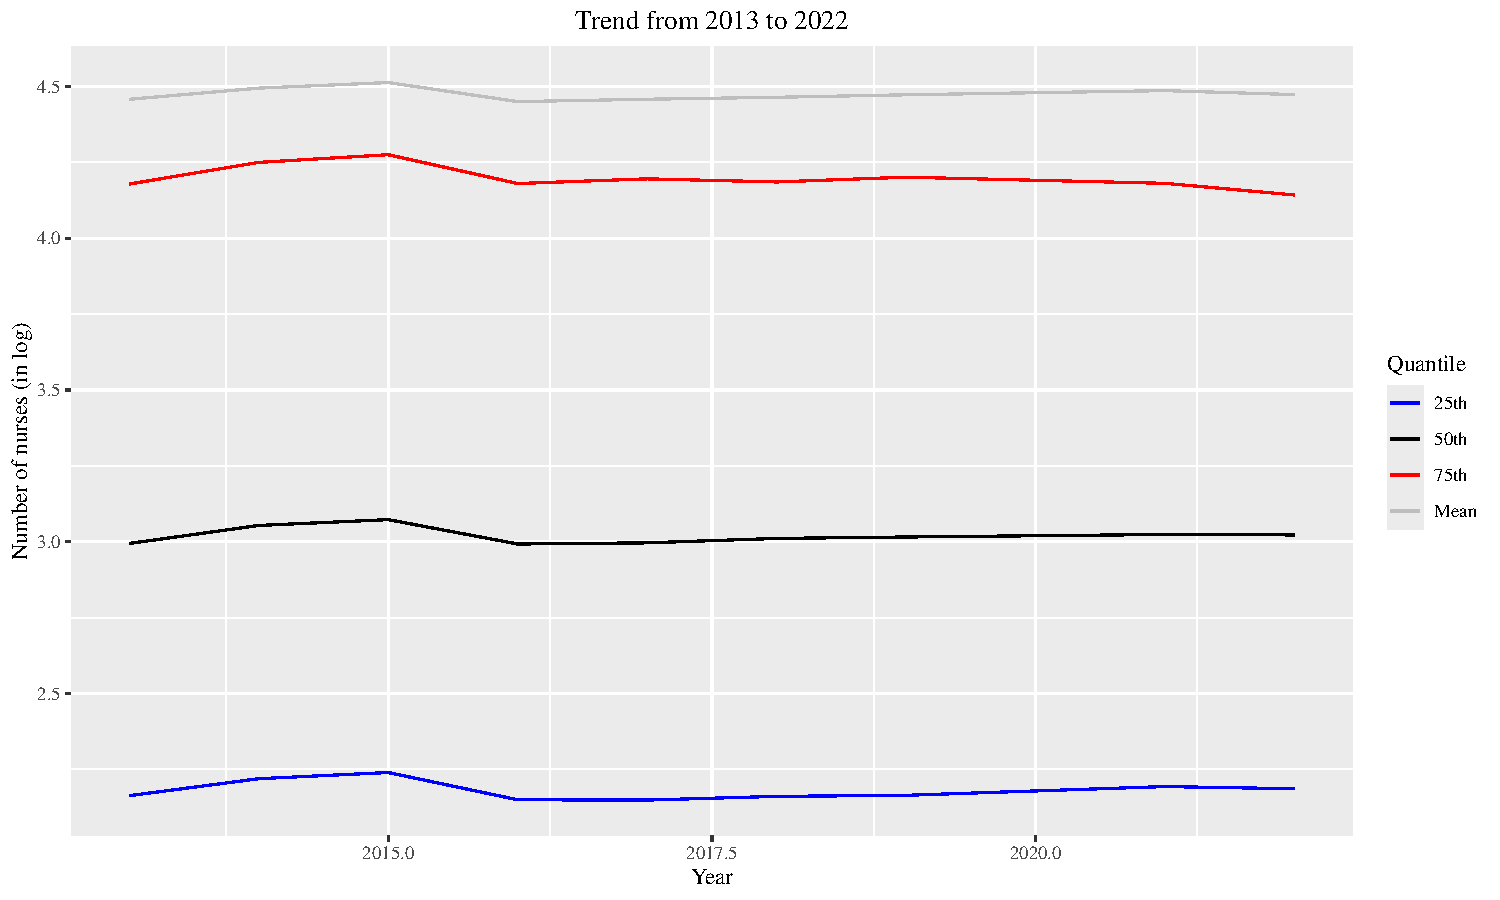
\includegraphics{../../Figures/Descriptive/nurses.pdf}
\end{adjustbox}

\subsection{Estimation (OLS)}

\footnote{On a side note, we filtered the panel such that
    \begin{enumerate}
        \item the number of nurses is positive,
        \item at least one of STAC inpatient, STAC outpatient, Sessions is positive,
        \item the number of observations is larger than 6
    \end{enumerate}}

\begin{table}
    
\begingroup
\centering
\begin{tabular}{lcccc}
   \tabularnewline \midrule \midrule
   Dependent Variable: & \multicolumn{4}{c}{Nurses}\\
                           & Pool          & Pool IV       & Dummy          & Dummy IV \\   
   Model:                  & (1)           & (2)           & (3)            & (4)\\  
   \midrule
   \emph{Variables}\\
   Constant                & 1.38$^{***}$  & 1.39$^{***}$  & 1.59$^{***}$   & 1.58$^{***}$\\   
                           & (0.022)       & (0.025)       & (0.025)        & (0.027)\\   
   STAC inpatient          & 0.282$^{***}$ & 0.279$^{***}$ & 0.277$^{***}$  & 0.276$^{***}$\\   
                           & (0.005)       & (0.005)       & (0.004)        & (0.005)\\   
   STAC outpatient         & 0.049$^{***}$ & 0.050$^{***}$ & 0.056$^{***}$  & 0.057$^{***}$\\   
                           & (0.003)       & (0.003)       & (0.003)        & (0.004)\\   
   Medical sessions        & 0.062$^{***}$ & 0.061$^{***}$ & 0.064$^{***}$  & 0.063$^{***}$\\   
                           & (0.002)       & (0.002)       & (0.002)        & (0.002)\\   
   External consultations  & 0.052$^{***}$ & 0.057$^{***}$ & 0.024$^{***}$  & 0.027$^{***}$\\   
                           & (0.001)       & (0.002)       & (0.002)        & (0.002)\\   
   Emergency               & 0.019$^{***}$ & 0.016$^{***}$ & 0.022$^{***}$  & 0.021$^{***}$\\   
                           & (0.001)       & (0.001)       & (0.001)        & (0.001)\\   
   Long-term \& follow-up  & 0.076$^{***}$ & 0.076$^{***}$ & 0.068$^{***}$  & 0.069$^{***}$\\   
                           & (0.002)       & (0.002)       & (0.002)        & (0.002)\\   
   Home care               & 0.018$^{***}$ & 0.016$^{***}$ & 0.027$^{***}$  & 0.026$^{***}$\\   
                           & (0.003)       & (0.003)       & (0.003)        & (0.003)\\   
   Psychiatric care        & 0.075$^{***}$ & 0.073$^{***}$ & 0.064$^{***}$  & 0.063$^{***}$\\   
                           & (0.003)       & (0.003)       & (0.003)        & (0.003)\\   
   Private Forprofit       &               &               & -0.282$^{***}$ & -0.270$^{***}$\\   
                           &               &               & (0.023)        & (0.027)\\   
   Private Nonprofit       &               &               & -0.198$^{***}$ & -0.180$^{***}$\\   
                           &               &               & (0.020)        & (0.021)\\   
   STJR0                   &               &               & 0.713$^{***}$  & 0.707$^{***}$\\   
                           &               &               & (0.020)        & (0.021)\\   
   \midrule
   \emph{Fit statistics}\\
   Observations            & 15,335        & 13,402        & 15,335         & 13,402\\  
   R$^2$                   & 0.820         & 0.821         & 0.837          & 0.838\\  
   \midrule \midrule
   \multicolumn{5}{l}{\emph{Heteroskedasticity-robust standard-errors in parentheses}}\\
   \multicolumn{5}{l}{\emph{Signif. Codes: ***: 0.01, **: 0.05, *: 0.1}}\\
\end{tabular}
\par\endgroup



\end{table}

\begin{table}
    
\begingroup
\centering
\begin{tabular}{lcccc}
   \tabularnewline \midrule \midrule
   Dependent Variable: & \multicolumn{4}{c}{log(ETP\_INF)}\\
                      & Teaching    & Public      & Forprofit   & Nonprofit \\   
   Model:             & (1)         & (2)         & (3)         & (4)\\  
   \midrule
   \emph{Variables}\\
   Constant           & 3.28$^{a}$  & 1.38$^{a}$  & 1.40$^{a}$  & 1.00$^{a}$\\   
                      & (0.328)     & (0.262)     & (0.095)     & (0.149)\\   
   log(SEJHC\_MCO)    & 0.108$^{b}$ & 0.331$^{a}$ & 0.261$^{a}$ & 0.344$^{a}$\\   
                      & (0.042)     & (0.048)     & (0.015)     & (0.034)\\   
   log(SEJHP\_MCO)    & 0.132$^{a}$ & 0.078$^{a}$ & 0.048$^{a}$ & 0.046$^{c}$\\   
                      & (0.032)     & (0.013)     & (0.011)     & (0.027)\\   
   log(SEANCES\_MED)  & 0.060$^{a}$ & 0.051$^{a}$ & 0.075$^{a}$ & 0.094$^{a}$\\   
                      & (0.020)     & (0.007)     & (0.006)     & (0.016)\\   
   log(CONSULT\_EXT)  & 0.017       & 0.025$^{a}$ & -0.003      & 0.001\\   
                      & (0.014)     & (0.008)     & (0.011)     & (0.012)\\   
   log(PASSU)         & 0.049$^{a}$ & -0.009      & 0.033$^{a}$ & 0.025$^{b}$\\   
                      & (0.011)     & (0.008)     & (0.005)     & (0.010)\\   
   log(ENTSSR)        & 0.058$^{a}$ & 0.052$^{a}$ & 0.057$^{a}$ & 0.118$^{a}$\\   
                      & (0.013)     & (0.008)     & (0.008)     & (0.019)\\   
   log(SEJ\_HAD)      & 0.022       & 0.028$^{a}$ & 0.049$^{a}$ & -0.011\\   
                      & (0.027)     & (0.007)     & (0.018)     & (0.022)\\   
   log(SEJ\_PSY)      & 0.026$^{b}$ & 0.070$^{a}$ & 0.084$^{a}$ & 0.045\\   
                      & (0.011)     & (0.010)     & (0.018)     & (0.046)\\   
   \midrule
   \emph{Fit statistics}\\
   Observations       & 1,123       & 5,260       & 4,415       & 2,604\\  
   R$^2$              & 0.779       & 0.860       & 0.742       & 0.754\\  
   \midrule \midrule
   \multicolumn{5}{l}{\emph{Clustered (FI) standard-errors in parentheses}}\\
   \multicolumn{5}{l}{\emph{Signif. Codes: a: 0.01, b: 0.05, c: 0.1}}\\
\end{tabular}
\par\endgroup



\end{table}

\subsection{Panel Data Estimator}
Though \cite{croiset2024hospitals} has mentioned that identification (and
significance level) is mainly attributed to \textit{between-group} variation,
there's still some level of \textit{within-group} variation that guarantee the
estimation of parameters.

\begin{table}
    \begin{tabular}{l c c}
    \toprule
                      & Within        & First Diff    \\
    \midrule
    log(SEJHC\_MCO)   & $0.099^{***}$ & $0.071^{***}$ \\
                      & $(0.004)$     & $(0.005)$     \\
    log(SEJHP\_MCO)   & $0.020^{***}$ & $0.015^{***}$ \\
                      & $(0.002)$     & $(0.002)$     \\
    log(SEANCES\_MED) & $0.023^{***}$ & $0.019^{***}$ \\
                      & $(0.002)$     & $(0.002)$     \\
    log(CONSULT\_EXT) & $0.002$       & $0.001$       \\
                      & $(0.001)$     & $(0.001)$     \\
    log(PASSU)        & $0.023^{***}$ & $0.013^{**}$  \\
                      & $(0.003)$     & $(0.004)$     \\
    log(ENTSSR)       & $0.013^{***}$ & $0.014^{***}$ \\
                      & $(0.002)$     & $(0.003)$     \\
    log(SEJ\_HAD)     & $0.014^{***}$ & $0.017^{***}$ \\
                      & $(0.004)$     & $(0.005)$     \\
    log(SEJ\_PSY)     & $0.002$       & $0.001$       \\
                      & $(0.001)$     & $(0.002)$     \\
    \midrule
    R$^2$             & $0.072$       & $0.031$       \\
    Num. obs.         & $15335$       & $13502$       \\
    \bottomrule
    \multicolumn{3}{l}{\scriptsize{$^{***}p<0.001$; $^{**}p<0.01$; $^{*}p<0.05$}}
\end{tabular}

\end{table}

\newpage
\bibliography{ref.bib}

\end{document}
